\documentclass[10pt]{beamer}

%%%
% PREAMBLE FOR THIS DOC 
%%%
%https://tex.stackexchange.com/questions/68821/is-it-possible-to-create-a-latex-preamble-header
\usepackage{/Users/miw267/Repos/csci246_fall2025/slides/preambles/beamer_preamble_for_CSCI246}



%%% TRY TO RESHOW TOC AT EACH SECTION START (with current section highlighted)
% Reference: https://tex.stackexchange.com/questions/280436/how-to-highlight-a-specific-section-in-beamer-toc
\newcommand\tocforsect[2]{%
  \begingroup
  \edef\safesection{\thesection}
  \setcounter{section}{#1}
  \tableofcontents[#2,currentsection]
  \setcounter{section}{\safesection}
  \endgroup
}


%%%% HERES HOW TO DO IT CORRECTLY
% FIRST IN .STY FILE, DO
%\usetheme[sectionpage=none]{metropolis}
% THEN AT EACH SECTION DO
%\begin{frame}{Outline}
%  \tableofcontents[currentsection]	
%\end{frame}



%\setbeamertemplate{navigation symbols}{}
%\setbeamertemplate{footline}[frame number]{}


%%% SPECIAL TO THIS DECK
\usepackage{adjustbox} % <--- for valign
\usetikzlibrary{arrows.meta,positioning}



%%%
% DOCUMENT
%%%

\begin{document}

%\maketitle

%% Title page frame
%\begin{frame}
%    \titlepage 
%\end{frame}





\title{09/21/2026: Set operations}
\author{CSCI 246: Discrete Structures}
\date{Textbook reference: Sec. 12, Scheinerman}

\begin{frame}
    \titlepage 
\end{frame}


\begin{frame}
\footnotesize 
%\begin{mygreenbox}[title=Graded Quiz Pickup]
%Quizzes are in the front of the room, grouped into four bins (A-G, H-L, M-R, S-Z) by last name. The quizzes are upside down with your last name on the back. Come find yours before, during, or after class.  Only turn the quiz over if it's yours.
%\end{mygreenbox} 
%\vfill 

%\begin{myredbox}[title=Announcements]
%
%\begin{itemize}
%\item  I still have lots of old quizzes; come pick them up.
%\item I will post the study guide to the slides after class.
%\item By default, I post slides to the course repo within the hour after class (5pm-6pm).  From here on, I will only announce about slide posting to Canvas if there is an exception.
%\item Please sign the attendance sheet.
%\end{itemize}
%
%\end{myredbox}
%
%\vfill 


\begin{myyellowbox}[title=Today's Agenda]
\begin{itemize}
	\item Review exercises ($\approx$ 10 mins)
	\item Mini-lecture ($\approx$ 25 mins)
	\item Group exercises ($\approx$ 15 mins)
\end{itemize}

\end{myyellowbox}
\vfill 

\end{frame}






\begin{frame}{Subtopics from today's reading}
Scheinerman Sec. 12 (Set Operations) covers the following subtopics
\begin{enumerate}
	\item Union and intersection
	\begin{enumerate}
	\item[a.] Introduction
 	\item[b.] Properties
 	\item[c.] The size of a union
 	\end{enumerate}
	\item Set Difference and Symmetric Difference
%	\begin{enumerate}
%	\item[a.] Introduction
%	\item[b.] Properties
% 	\end{enumerate}
	\item Cartesian Product 
\end{enumerate}

\end{frame}


%%%% Section
\begin{frame}[standout]
Outline for Mini-Lecture:
\begin{itemize}
\item \alert{\textbullet \quad Union and Intersection}
\item \alert{\quad \textopenbullet \quad Introduction}
\item \quad \textopenbullet \quad Properties
\item \quad \textopenbullet \quad Size of a Union
\item \textbullet \quad Set \& Symmetric Difference 
\item \textbullet \quad Cartesian Product
\end{itemize}
\end{frame}



\begin{frame}{Union and Intersection}

Let $A$ and $B$ be sets.
\vspace{.1cm}

\colorbox{green!30}{\textbf{Definition.}} The \textbf{union} of $A$ and $B$, denoted $A \cup B$ is the set of all elements that are in $A$ or $B$ (or both).

\begin{center}
\begin{tabular}{c c}
  \adjustbox{valign=c}{$A \cup B = \{x : x \in A \text{ or } x \in B\}$} &
  \adjustbox{valign=c}{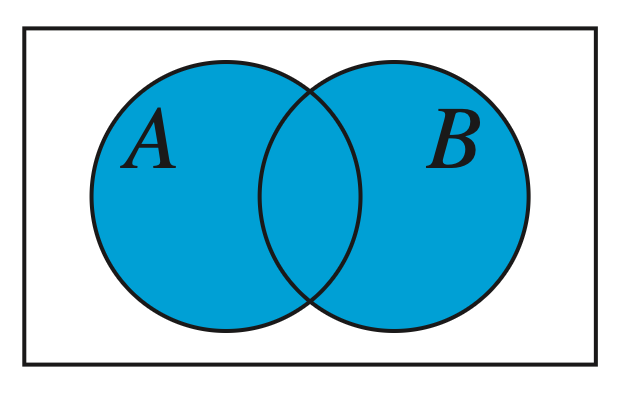
\includegraphics[width=.25\textwidth]{images/union.png}} \\
\end{tabular}
\end{center}


\vfill 
\pause 

\colorbox{green!30}{\textbf{Definition.}} The \textbf{intersection} of $A$ and $B$, denoted $A \cap B$ is the set of all elements that are in both $A$ and $B$.

\begin{center}
\begin{tabular}{c c}
  \adjustbox{valign=c}{$ A \cap B = \set{x : x \in A \text{ and } x \in B}$} &
  \adjustbox{valign=c}{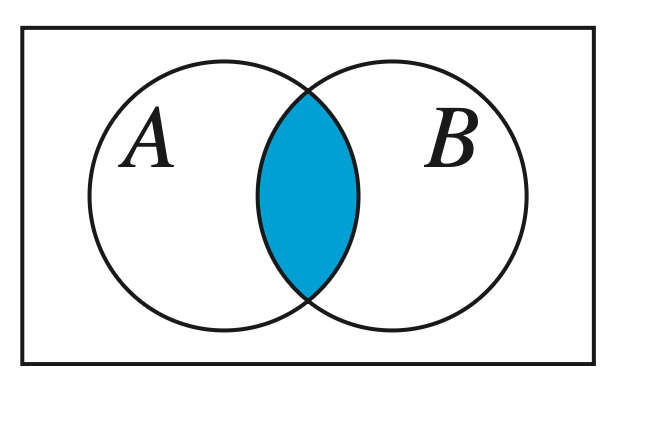
\includegraphics[width=.25\textwidth]{images/intersection.png}} \\
\end{tabular}
\end{center}

\end{frame}


\begin{frame}{Union and Intersection: Emoji Math}

\newcommand{\happy}{\adjustbox{valign=c}{
\includegraphics[height=3em]{images/happy}}}
\newcommand{\mad}{\adjustbox{valign=c}{
\includegraphics[height=3em]{images/mad}}}
\newcommand{\poop}{\adjustbox{valign=c}{
\includegraphics[height=3em]{images/poop}}}
\newcommand{\wind} {\adjustbox{valign=c}{
\includegraphics[height=3em]{images/wind}}}
\newcommand{\tornado} {\adjustbox{valign=c}{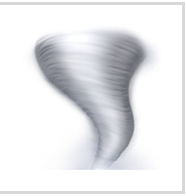
\includegraphics[height=3em]{images/tornado}}}


\begin{align*}
F &= \bigg\{\happy, \mad \bigg\} && \text{face emojis}\\
N &= \bigg\{\mad, \poop \bigg\} && \text{negative emojis}\\
 \onslide<2->{F \cap N &= \bigg\{\mad \bigg\} && \text{negative face emojis}} \\
 \onslide<3->{F \cup N &= \bigg\{\happy, \mad, \poop \bigg\} && \text{face or negative emojis}} \\
\end{align*}

	
\end{frame}


%%%% Section
\begin{frame}[standout]
Outline for Mini-Lecture:
\begin{itemize}
\item \alert{\textbullet \quad Union and Intersection}
\item \quad \textopenbullet \quad Introduction
\item \alert{\quad \textopenbullet \quad Properties}
\item \quad \textopenbullet \quad Size of a Union
\item \textbullet \quad Set \& Symmetric Difference 
\item \textbullet \quad Cartesian Product
\end{itemize}
\end{frame}


\begin{frame}{Union and Intersection Properties}

\newcommand{\happy}{\adjustbox{valign=c}{
\includegraphics[height=2em]{images/happy}}}
\newcommand{\mad}{\adjustbox{valign=c}{
\includegraphics[height=2em]{images/mad}}}
\newcommand{\poop}{\adjustbox{valign=c}{
\includegraphics[height=2em]{images/poop}}}
\newcommand{\wind} {\adjustbox{valign=c}{
\includegraphics[height=2em]{images/wind}}}
\newcommand{\tornado} {\adjustbox{valign=c}{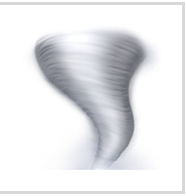
\includegraphics[height=2em]{images/tornado}}}

\small 

\colorbox{blue!30}{\textbf{Overview.}} Set operations have many properties.  E.g. the \alert{distributive properties} are:


\[ A \cup (B \cap C) = (A \cup B) \cap (A \cup C),\qquad  A \cap (B \cup C) = (A \cap B) \cup (A \cap C) \]

\vfill 

\colorbox{green!30}{\textbf{Intuition.}} Let's apply the lefthand property to  wind emojis $W$, face emojis $F$, and negative emojis $N$.  %So we aim to show
%\[ W \cup (F \cap N) = (W \cup F) \cap (W \cup N) \]
\vfill 
\vspace{-.2cm}
\begin{align*}
&W \cup (F \cap N) \\
&= \big\{\wind, \tornado \big\} \bigcup \bigg( \; \big\{\mad, \happy \big\} \bigcap \big\{\mad, \poop \big\} \; \bigg) 	\\
&= \big\{\wind, \tornado \big\} \bigcup \big\{\mad \big\} 	\\
&=\big\{\wind, \tornado, \mad \big\}  \\
&=\big\{\wind, \tornado, \mad, \happy \big\}  \bigcap  \big\{\wind, \tornado, \mad, \poop \big\}  \\
&=\bigg( \big\{\wind, \tornado\big\} \bigcup \big\{\mad, \happy \big\} \bigg) \bigcap  \bigg( \big\{\wind, \tornado\big\} \bigcup \big\{\mad, \poop \big\}  \bigg) \\
&=(W \cup F) \cap (W \cup N)
\end{align*}

\end{frame}




\begin{frame}{Union and Intersection Properties}

\colorbox{green!30}{\textbf{Intuition.}}
We can also build intuition about the set properties by creating an application.

\vfill 
\pause 

\begin{minipage}{0.82\textwidth}
Suppose we work for Rosauers and we are studying how likely customers are to make a purchase in different parts of the store.   Let
\end{minipage} %
  \hfill
    \begin{minipage}{0.15\textwidth}
  % image sized to 2em and vertically centered
  \adjustbox{valign=c}{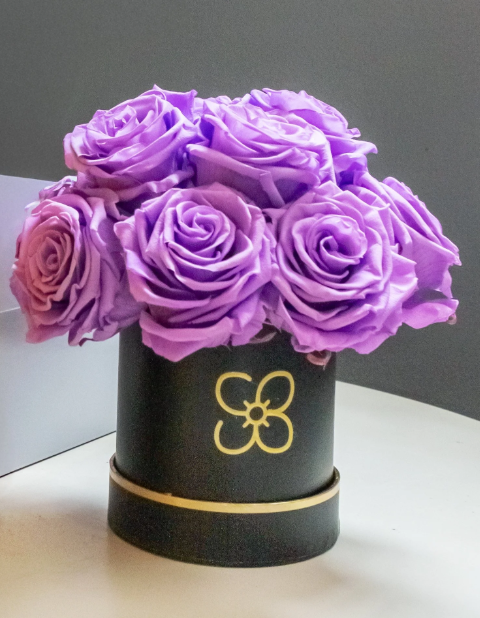
\includegraphics[height=3em]{images/roses}}
\end{minipage}%
    
	\begin{itemize}
	\item $P$: The set of Rosauers customers who made a purchase. 
	\item $R$: The set of Rosauers customers who were shopping for roses.
	\item $C$: The set of Rosauers customers who were shopping for candy.
	\end{itemize}
	
Then
\[ (R \cup C)  \cap P \explaintermbrace{commutative}{=}  P \cap (R \cup C) \explaintermbrace{distributive }{=} (P \cap R) \cup (P \cap C). \]


\vfill 
\pause 

\colorbox{yellow!30}{\textbf{Poll.}} What does this equation say?  \pause  The set of Rousauers customers who were shopping for roses or candy and made a purchase is the same as the set of Rosauers customers who were shopping for roses and made a purchase combined with the set of Rosauers customers who were shopping for candy and made a purchase.
	
\end{frame}

\begin{frame}{Union and Intersection Properties: Proofs}
\small 
\colorbox{yellow!30}{\textbf{Poll.}} How would we go about \alert{proving} a set property -- e.g. the first distributive property?
\[ A \cup (B \cap C) = (A \cup B) \cap (A \cup C) \]

\vfill 
\pause 
\colorbox{blue!30}{\textbf{Strategy.}} Recall that the definitions of union and intersection depends upon logical operators \red{\textbf{and}} and \red{\textbf{or}}

\begin{align*}
A \cup B &= \{x : x \in A \red{\textbf{ or }} x \in B\} \\
A \cap B &= \{x : x \in A \red{\textbf{ and }} x \in B\} \\
\end{align*}

\vfill 
\pause 
\vspace{-.8cm}
Thus, we can rely upon the analogous properties from \alert{Boolean algebra} to do all the heavy lifting.
\vfill 
\pause 
\vspace{-.3cm}
\begin{center}

\includegraphics[width=.8\textwidth]{images/boolean_algebra_properties} \\
\textit{Do you remember the Boolean Algebra props. (Theorem 7.2)?!}
\end{center}
\end{frame}



\begin{frame}{Union and Intersection Properties: Proofs}
\footnotesize
\colorbox{red!30}{\textbf{Problem.}}  The distributive properties for sets are 
    \[ A \cup (B \cap C) = (A \cup B) \cap (A \cup C), \qquad \text{and} \qquad  A \cap (B \cup C) = (A \cap B) \cup (A \cap C). \]
Prove that the first identity above holds.  
\vfill 
\pause  

\colorbox{green!30}{\textbf{Solution.}}  

\begin{align*}
 \onslide<3->{A \cup (B \cap C) &= \set{x: x \in A \text{ or } x \in B \cap C} && \scripttext{(by def. union $\cup$)}} \\
 \onslide<4->{&= \set{x: x \in A \text{ or } (x \in B \text{ and }  x \in C) } && \scripttext{(by def. intersection $\cap$)}} \\
 \onslide<5->{&= \set{x: (x \in A \text{ or } x \in B) \text{ and }  (x \in A \text{ or } x \in C) } && \scripttext{\alert{(by distributive prop.; Thm 7.2)}}} \\
 \onslide<6->{&= \set{x: (x \in A \cup B) \text{ and }  (x \in A \cup C)} && \scripttext{(by def. union $\cup$)}} \\
 \onslide<7->{&= (A \cup B) \cap (A \cup C) && \scripttext{(by def. intersection $\cap$)}}
\end{align*}

 \onslide<8->{\colorbox{blue!30}{\textbf{Remark.}}   We used the \alert{distributive property for \textit{Boolean Algebra} (from Theorem 7.2)} to prove the distributive property for \textit{sets}.}
\end{frame}



\begin{frame}{Union and Intersection Properties: Visual Intuition}

\textbf{Venn diagrams} are also useful for understanding set properties.

\vfill 
\pause 
\colorbox{yellow!30}{\textbf{Poll.}}  How does the digram below illustrate the distributive property

    \[ A \cup (B \cap C) = (A \cup B) \cap (A \cup C) \]
    
 \vfill 
 
 \begin{center}
 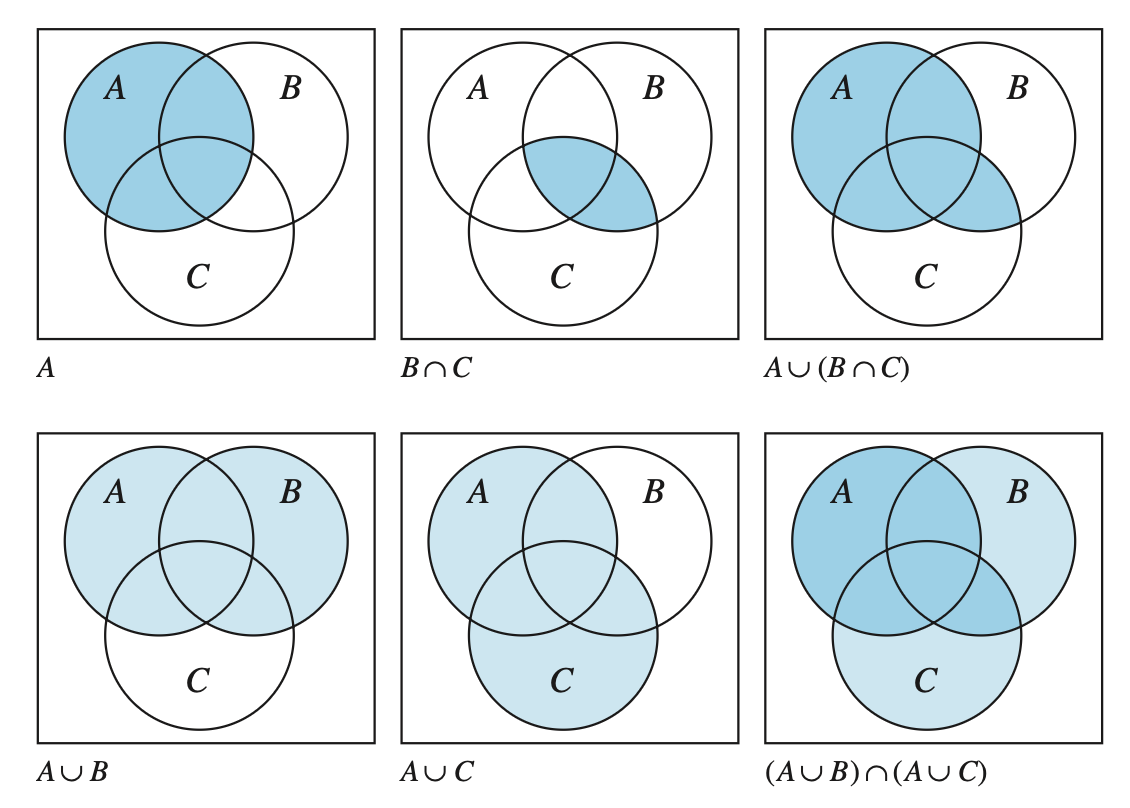
\includegraphics[width=.775\textwidth]{images/venn_distributive}
 \end{center}

\end{frame}

\begin{frame}{Union and Intersection Properties}

A complete set of properties related to set union and intersections is given in the text.

 \begin{center}
 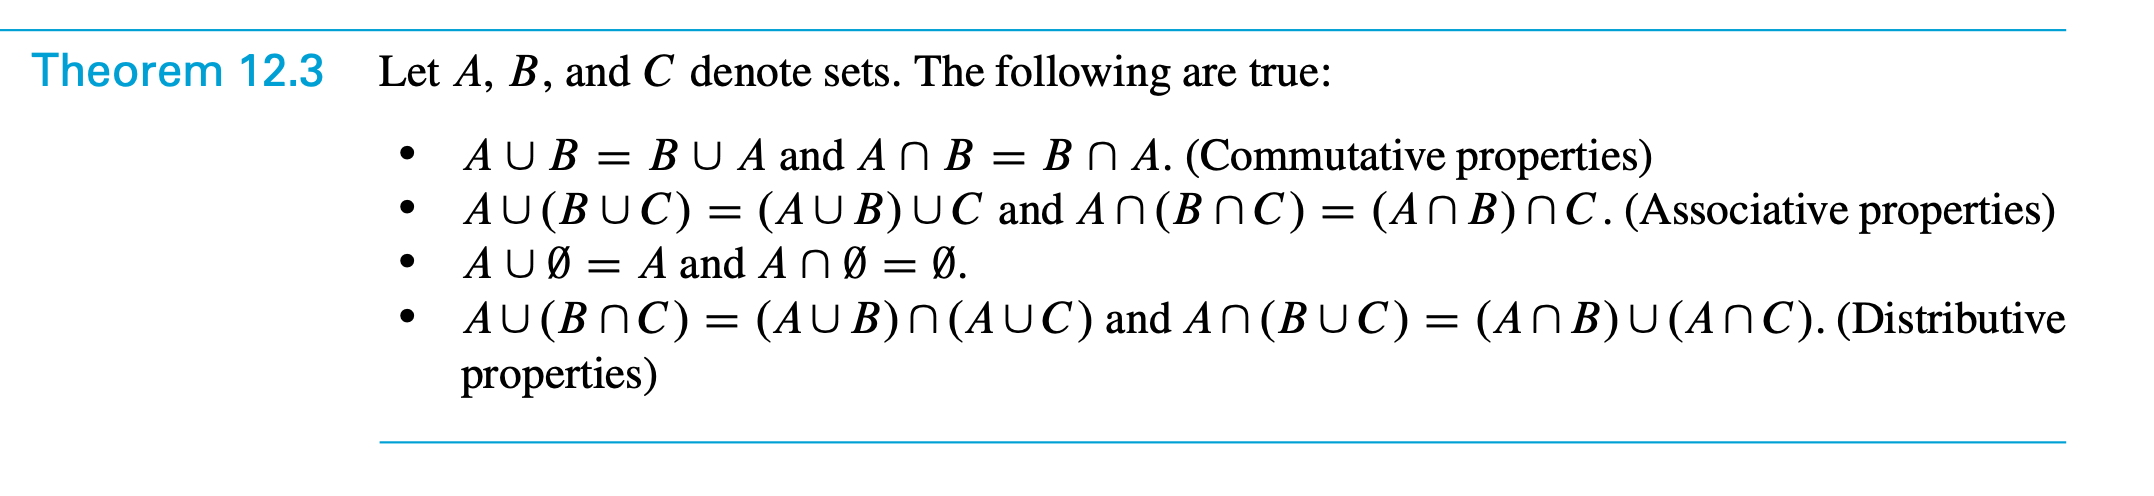
\includegraphics[width=\textwidth]{images/union_intersection_properties_text}
 \end{center}



	
\end{frame}


%%%% Section
\begin{frame}[standout]
Outline for Mini-Lecture:
\begin{itemize}
\item \alert{\textbullet \quad Union and Intersection}
\item \quad \textopenbullet \quad Introduction
\item \quad \textopenbullet \quad Properties
\item \alert{\quad \textopenbullet \quad Size of a Union}
\item \textbullet \quad Set \& Symmetric Difference 
\item \textbullet \quad Cartesian Product
\end{itemize}
\end{frame}


\begin{frame}{The Size of a Union}
\small 

\colorbox{yellow!30}{\textbf{Poll.}} Discuss what $|A \cup B | = |A| + |B|$ means. Is it correct?

\vfill 
\pause 
\colorbox{green!30}{\textbf{Solution.}} No! It's correct only when $A \cap B = \emptyset$. (That is, when $A$ and $B$ are \textbf{disjoint} -- i.e. they have no elements in common.)  \pause \colorbox{yellow!30}{\textbf{Poll.}} Why? \pause 

% \pause  \colorbox{green!30}{\textbf{Solution.}}  The correct equation for the size of a union is 

%\begin{tcolorbox}[colback=green!20, colframe=black, boxrule=0.5pt]
%\[ |A \cup B | = |A| + |B| - |A \cap B|\] 
%\end{tcolorbox}

\begin{mygreenbox}[title=\text{The Size of a Union (Scheinerman Prop 12.4)}]
Let $A$ and $B$ be finite sets. Then
\[ |A \cup B | = |A| + |B| - |A \cap B|\] 
\end{mygreenbox}


\vfill

\begin{center}
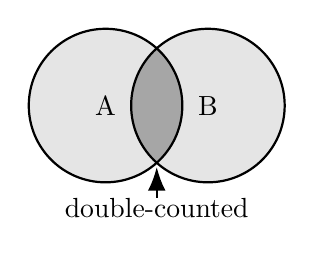
\begin{tikzpicture}[scale=0.65]

  % Light shading for union (A or B)
  \fill[gray!20] (0,0) circle (1.5);
  \fill[gray!20] (2,0) circle (1.5);

  % Heavy shading for intersection
  \begin{scope}
    \clip (0,0) circle (1.5);
    \fill[gray!70] (2,0) circle (1.5);
  \end{scope}

  % Outlines
  \draw[thick] (0,0) circle (1.5);
  \draw[thick] (2,0) circle (1.5);

  % Labels inside the circles
  \node at (0,0) {A};
  \node at (2,0) {B};

  % Arrow pointing upward at the intersection
  \draw[-{Latex[length=3mm]}, thick] 
    (1,-1.8) -- (1,-1.2);

  % Labels below arrow
  \node at (1,-2.0) {double-counted};

\end{tikzpicture}
\end{center}

\vfill 
\pause 

\colorbox{yellow!30}{\textbf{Poll.}} When is this equation useful?  \pause  \colorbox{green!30}{\textbf{Solution.}} When  computing $|A|,|B|, |A \cap B|$ is easier than $|A \cup B|$. \pause (Example: Today's Group Exercise \#4.)
\end{frame}




%%%% Section
\begin{frame}[standout]
Outline for Mini-Lecture:
\begin{itemize}
\item \textbullet \quad Union and Intersection
\item \alert{\textbullet \quad Set \& Symmetric Difference}
\item \textbullet \quad Cartesian Product
\end{itemize}
\end{frame}

\begin{frame}{Set and Symmetric Difference}
	
Let $A$ and $B$ be sets.
\vspace{.1cm}

\colorbox{green!30}{\textbf{Definition.}} The \textbf{set difference} of $A$ and $B$, denoted $A - B$ is the set of all elements that are in $A$ but not in $B$.

\begin{center}
\begin{tabular}{c c}
  \adjustbox{valign=c}{$A - B = \{x : x \in A \text{ and } x \not\in B\}$} &
  \adjustbox{valign=c}{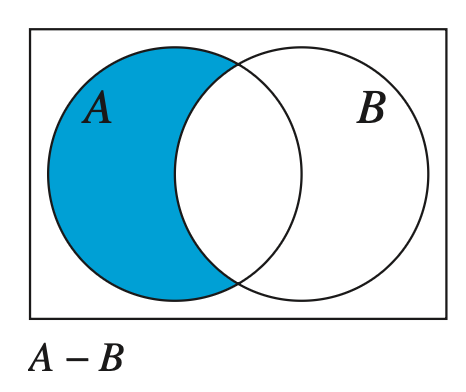
\includegraphics[width=.25\textwidth]{images/set_difference.png}} \\
\end{tabular}
\end{center}


\vfill 
\pause 

\colorbox{green!30}{\textbf{Definition.}} The \textbf{symmetric difference} of $A$ and $B$, denoted $A \; \triangle \; B$ is the set of all elements that are in $A$ but not $B$ or $B$ but not $A$.

\begin{center}
\begin{tabular}{c c}
  \adjustbox{valign=c}{$ A \; \triangle \; B = (A - B) \cup (B - A)$} &
  \adjustbox{valign=c}{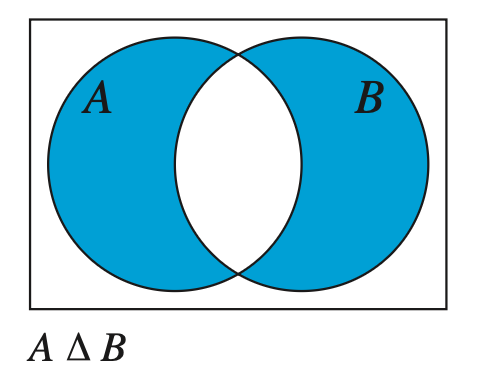
\includegraphics[width=.25\textwidth]{images/symmetric_difference.png}} \\
\end{tabular}
\end{center}

\end{frame}


\begin{frame}{Set and Symmetric Difference: Emoji Math}

\newcommand{\happy}{\adjustbox{valign=c}{
\includegraphics[height=3em]{images/happy}}}
\newcommand{\mad}{\adjustbox{valign=c}{
\includegraphics[height=3em]{images/mad}}}
\newcommand{\poop}{\adjustbox{valign=c}{
\includegraphics[height=3em]{images/poop}}}
\newcommand{\wind} {\adjustbox{valign=c}{
\includegraphics[height=3em]{images/wind}}}
\newcommand{\tornado} {\adjustbox{valign=c}{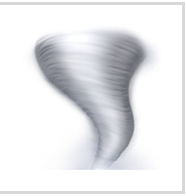
\includegraphics[height=3em]{images/tornado}}}


\begin{align*}
F &= \bigg\{\happy, \mad \bigg\} && \text{face emojis}\\
N &= \bigg\{\mad, \poop \bigg\} && \text{negative emojis}\\
\onslide<2->{F - N &= \bigg\{\happy \bigg\} && \text{happy face emojis}} \\
\onslide<3->{F \triangle N &= \bigg\{\happy,  \poop \bigg\} && \text{non-negative face and non-face negative emojis}} 
\end{align*}

\end{frame}

\begin{frame}{Symmetric Difference: Alternate Characterization}

\begin{mygreenbox}[title=\text{A characterization of symmetric difference (Scheinerman Prop 12.11)}]
Let $A$ and $B$ be sets. Then
\[ A \; \triangle \; B = (A \cup B) - (A \cap B) \]
\end{mygreenbox}

\vfill 

\pause 

\colorbox{blue!30}{\textbf{Visual Intuition.}}
\begin{center}
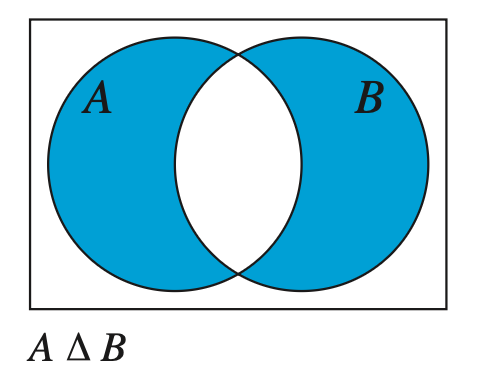
\includegraphics[width=.25\textwidth]{images/symmetric_difference.png}
\end{center}

\end{frame}


\begin{frame}{Symmetric Difference: Alternate Characterization}

\begin{mygreenbox}[title=\text{A characterization of symmetric difference (Scheinerman Prop 12.11)}]
Let $A$ and $B$ be sets. Then
\[ A \; \triangle \; B = (A \cup B) - (A \cap B) \]
\end{mygreenbox}


\colorbox{yellow!30}{\textbf{Poll.}} How could we prove this is true?

\vfill 
\pause 
\begin{myredbox}[title=\text{Reminder from Sec. 10: Proving two sets are equal}]
To show $S=T$, we show $S \subseteq T$ and $T \subseteq S$.
\begin{itemize}
\item $\boxed{S \subseteq T.}$ We show that if $x \in S $, then $x \in T$.    \only<3-4>{\quad \red{In this case, we show that if $x \in A \; \triangle \; B$, then $x \in (A \cup B) - (A \cap B)$.}}
\item $\boxed{T \subseteq S.}$	We show that if $x \in T$, then $x \in S$. \only<4>{\quad \red{In this case, we show that if $x \in (A \cup B) - (A \cap B)$, then $x \in A \; \triangle \; B$.}}
\end{itemize}
\end{myredbox}
\vfill 
\pause 

\colorbox{blue!30}{\textbf{Remark.}} For details, see the textbook.

\end{frame}


\begin{frame}{DeMorgan's Law}
The textbook gives DeMorgan's Law as

\begin{center}
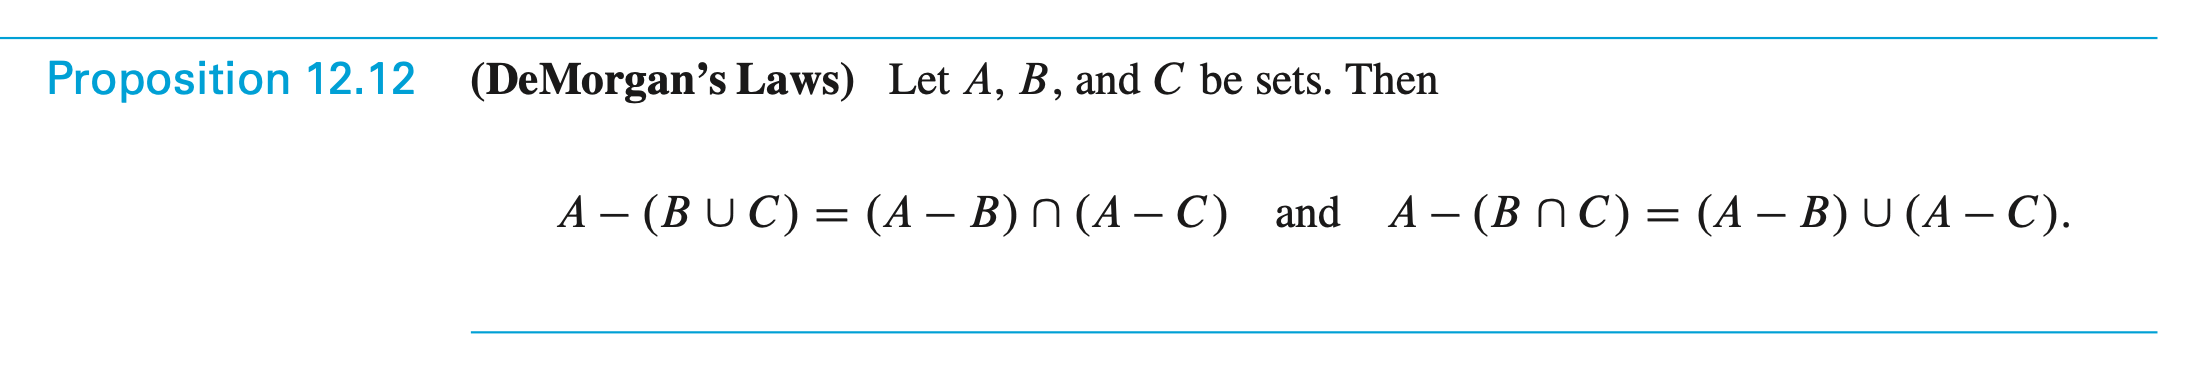
\includegraphics[width=\textwidth]{images/demorgan_text.png}	
\end{center}

\vfill \pause 
\colorbox{blue!30}{\textbf{Remark.}} A simpler way to express this law is as follows. Let $X$ be a \qq{universe}; that is, every element we consider is in $X$.  For any set $S$, define its \textbf{complement} $\overline{S}$ as points not in $S$ (but in X).  Then we can write DeMorgan's Law as 

\[ \overline{A \cup B} = \overline{A} \cap \overline{B}, \qquad \overline{A \cap B} = \overline{A} \cup \overline{B}\]

\vfill
\pause 
\vspace{-.5cm}
That is, 
\begin{itemize}
	\item The complement of the union of two sets is the same as the intersection of their complements.
\item The complement of the intersection of two sets is the same as the union of their complements
\end{itemize}

\end{frame}



%%%% Section
\begin{frame}[standout]
Outline for Mini-Lecture:
\begin{itemize}
\item \textbullet \quad Union and Intersection
\item \textbullet \quad Set \& Symmetric Difference
\item \alert{\textbullet \quad Cartesian Product}
\end{itemize}
\end{frame}

\begin{frame}{Cartesian Product}
	
Let $A$ and $B$ be sets.
\vspace{.1cm}

\colorbox{green!30}{\textbf{Definition.}} The \textbf{Cartesian product} of $A$ and $B$, denoted $A \times B$ is the set of all ordered pairs (two element lists) formed by taking an element of $A$ together with an element from $B$ in all possible ways.

 \[A \times B = \{ (a,b) : a \in A, b \in B\} \]

\end{frame}


\begin{frame}{Cartesian Product: Emoji Math}

\newcommand{\happy}{\adjustbox{valign=c}{
\includegraphics[height=3em]{images/happy}}}
\newcommand{\mad}{\adjustbox{valign=c}{
\includegraphics[height=3em]{images/mad}}}
\newcommand{\poop}{\adjustbox{valign=c}{
\includegraphics[height=3em]{images/poop}}}
\newcommand{\wind} {\adjustbox{valign=c}{
\includegraphics[height=3em]{images/wind}}}
\newcommand{\tornado} {\adjustbox{valign=c}{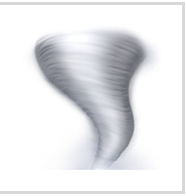
\includegraphics[height=3em]{images/tornado}}}


\begin{align*}
F &= \bigg\{\happy, \mad \bigg\} && \text{face emojis}\\
N &= \bigg\{\mad, \poop \bigg\} && \text{negative emojis} 
\end{align*}

\pause 

\begin{align*}
F \times N&= \Bigg\{ \bigg(\happy, \mad\ \bigg), \bigg(\happy, \poop\bigg), \\
 & \qquad \bigg(\mad, \mad\bigg), \bigg(\mad, \poop \bigg) \Bigg\} 
\end{align*}

\vfill 
\pause 

So $F \times N$ is a face emoji paired with a negative emoji. 

\vfill 
\pause 

\colorbox{blue!30}{\textbf{Remark.}} $F \times N \neq N \times F$.

\end{frame}


\begin{frame}{Application: Database management}
\footnotesize 
One application of set theory in computer science is in \textbf{database management systems} (DBMS), particularly in \textbf{SQL query optimization}.
\vfill 

\begin{mygreenbox}[title=Example]
Imagine a company has two database tables:

\begin{itemize}
\item \textbf{Customers} (Set $C$): Contains all registered customers.
\item \textbf{Orders} (Set $O$): Contains all customer orders.
\end{itemize}

A database query like:
\vspace{-.25cm}
\begin{center}
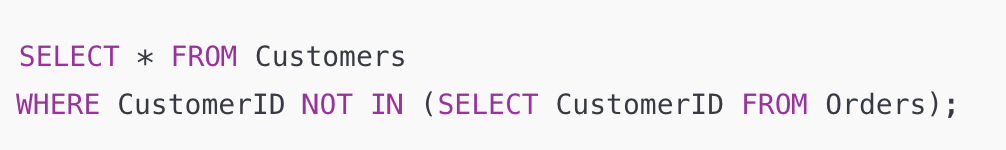
\includegraphics[width=.6\textwidth]{images/sql_query.png}	
\end{center}
\vspace{-.25cm}
is using the set difference $C-O$ to find customers who have never placed an order.
\end{mygreenbox}
\vfill

\begin{myyellowbox}[title=Key Set Operations in Databases]
\begin{itemize}
\item  Union ($A \cup B$)  $\to$ \texttt{UNION} in SQL (Combining results from multiple queries)
\item  Intersection ($A \cap B$)  $\to$ \texttt{INTERSECT} in SQL  (Finding common data between queries)
\item  Set Difference ($A - B$)  $\to$ \texttt{EXCEPT}  or \texttt{NOT IN} in SQL (Finding items in one table but not the other)	
\end{itemize}
\end{myyellowbox}


\end{frame}


\begin{frame}{Random group assignments}
\begin{columns}
\begin{column}{0.33\textwidth}
Ashley, Isabelle: 4 \\ 
Bailey, Tanna: 9 \\ 
Blaisdell, Olyver: 11 \\ 
Brown, Ashton: 6 \\ 
Brown, Jonathan: 10 \\ 
Cardenas, Dominic: 13 \\ 
Cutler, George: 13 \\ 
Fabik, Roland: 3 \\ 
Fellows, Audrey: 7 \\ 
Fitzgerald, Ryan: 10 \\ 
Fuller, Ryan: 7 \\ 
Griffen, Clara: 10 \\ 
Grutsch, Tanner: 1 \\\end{column}
\begin{column}{0.33\textwidth}
Hager, Nathan: 2 \\ 
Horner, Jayden: 5 \\ 
Johnson, Jaret: 8 \\ 
Kintzel, Samantha: 5 \\ 
Lameres, Alexis: 4 \\ 
Lee, Holden: 8 \\ 
Mayala, Reece: 7 \\ 
McLean, Connor: 5 \\ 
Mcbride, Daniel: 13 \\ 
Miller, Maverick: 11 \\ 
Moss, Emily: 1 \\ 
Mousseau, Matthew: 9 \\ 
Neuman, Evan: 9 \\\end{column}
\begin{column}{0.33\textwidth}
Putnam, John: 6 \\ 
Ramos, Vydel: 6 \\ 
Rathbun, Jedidiah: 8 \\ 
Roberts, Matthew: 12 \\ 
Roller, Nathan: 3 \\ 
Ryan, Otis: 3 \\ 
Shevtsov, Timothy: 2 \\ 
Sinclair, Aidan: 2 \\ 
Smith, Charles: 12 \\ 
Stensland, Emma: 4 \\ 
Thiessen, Logan: 12 \\ 
Thompson, Jaiden: 1 \\ 
Vath, Ethan: 11 \\\end{column}
\end{columns}
\end{frame}

\begin{frame}{Group Exercises: Set Operations}

\footnotesize 
\begin{enumerate}
	\item Let $A=\set{1,2,3,4,5}$ and $B=\set{4,5,6,7}$. Please compute (a) $A \cup B$, (b) $A \cap B$, (c) $A - B$, (d) $B-A$, (e) $A \, \triangle \, B$, (f) $A \times B$, and (g)  $B \times A$.
    \item The distributive properties for sets are 
    \[ A \cup (B \cap C) = (A \cup B) \cap (A \cup C), \qquad \text{and} \qquad  A \cap (B \cup C) = (A \cap B) \cup (A \cap C). \]
    The Venn diagram below illustrates the first distributive property. Make a Venn diagram to illustrate the second distributive property.
    \begin{center}
    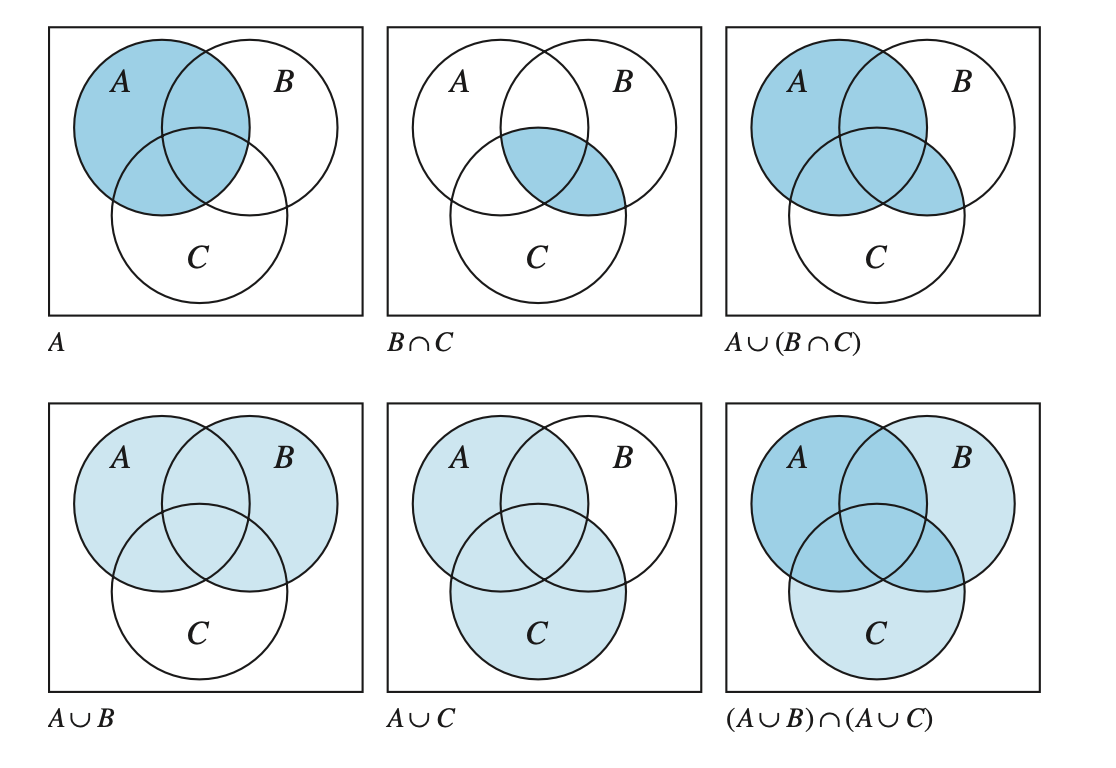
\includegraphics[width=.5\textwidth]{images/set_distributive_property}
    \end{center} 
    \item Prove that the second identity in \#2 holds.  \textit{Hint}: Use Theorem 7.2 (Boolean algebra properties).
    \item How many integers in the range 1 to 1000 (inclusive) are divisible by 2 or by 5?  Justify your answer. \textit{Hint:} Use Proposition 12.4 (Size of a Union).
\end{enumerate}
\end{frame}

\begin{frame}{Solution to Group Exercise \#1 (a-e) }

\colorbox{red!30}{\textbf{Problem.}} Let $A=\set{1,2,3,4,5}$ and $B=\set{4,5,6,7}$. Please compute (a.) $A \cup B$, (b.) $A \cap B$, (c.) $A - B$, (d.) $B-A$, and (e.) $A \, \triangle \, B$.\\
\vfill 
\colorbox{green!30}{\textbf{Solution.}}
   \begin{itemize}
        \item[(a.)] $A \cup B = \set{1,2,3,4,5,6,7}$.
        %\textit{Explanation.} The union is set of elements in either $A$ or $B$.
        \item[(b.)] $A \cap B = \set{4,5}$.  %\textit{Explanation.} The intersection is set of elements in both $A$ and $B$.
        \item[(c.)] $A - B = \set{1,2,3}$.
        \item[(d.)] $B-A = \set{6,7}$.
        \item[(e.)] $A \, \triangle \, B = \set{1,2,3,6,7}$. [Note:  $A \, \triangle \, B = (A-B) \cup (B-A)$.]
    \end{itemize}

\end{frame}

\begin{frame}{Solution to Group Exercise \#1 (f-g) }

\footnotesize 
\colorbox{red!30}{\textbf{Problem.}} Let $A=\set{1,2,3,4,5}$ and $B=\set{4,5,6,7}$. Please compute (f.) $A \times B$ and (g.)  $B \times A$.\\

\colorbox{green!30}{\textbf{Solution.}}
   \begin{itemize}
        \item[(f.)]    
        \begin{align*}
	A \times B = \bigg\{ & (1,4),(1,5),(1,6),(1,7), \\
	& (2,4),(2,5),(2,6),(2,7), \\
& (3,4),(3,5),(3,6),(3,7), \\
 & (4,4),(4,5),(4,6),(4,7), \\
& (5,4),(5,5),(5,6),(5,7)    \bigg\}    	
    \end{align*}
        \item[(g.)]    
        \begin{align*}
	B \times A = \bigg\{ & (4,1),(4,2),(4,3),(4,4), (4,5) \\
 & (5,1),(5,2),(5,3),(5,4), (5,5) \\
 & (6,1),(6,2),(6,3),(6,4), (6,5) \\
& (7,1),(7,2),(7,3),(7,4), (7,5)   \bigg\}   
    \end{align*}
    \end{itemize}
    
\end{frame}


\begin{frame}{Solution to Group Exercise \#2 }
\footnotesize 
\textbf{Problem.} The distributive properties for sets are 
    \[ A \cup (B \cap C) = (A \cup B) \cap (A \cup C), \qquad \text{and} \qquad  A \cap (B \cup C) = (A \cap B) \cup (A \cap C). \]
 Make a Venn diagram to illustrate the second distributive property.
 \vfill 
\textbf{Solution.}
	\scalebox{0.5}{  % Scale everything down 
        \begin{tabular}{ccc}   % Create a 2x3 grid
        % First Venn Diagram
        \Huge \textbf{$A$} &         \Huge \textbf{$B \cup C$}  &        \Huge \textbf{$A \cap (B \cup C)$} \\
        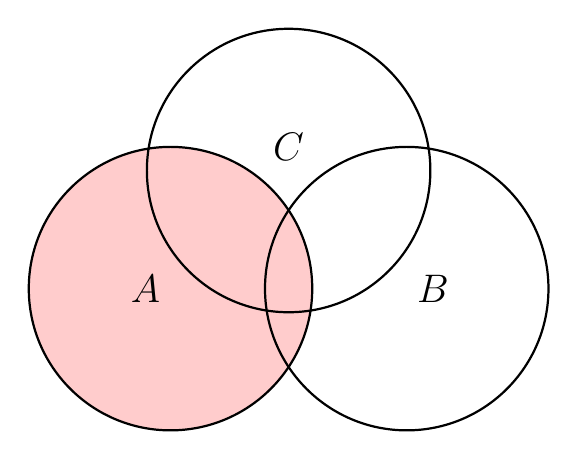
\begin{tikzpicture}
             \fill[red!20] (-1.5,0) circle (1.8);  % Set A (shaded)
            \draw[thick] (-1.5,0) circle (1.8) node[left] {\Large \( A \)};
            \draw[thick] (1.5,0) circle (1.8) node[right] {\Large \( B \)};
            \draw[thick] (0,1.5) circle (1.8) node[above] {\Large \( C \)};
        \end{tikzpicture}
        &
        % Second Venn Diagram
        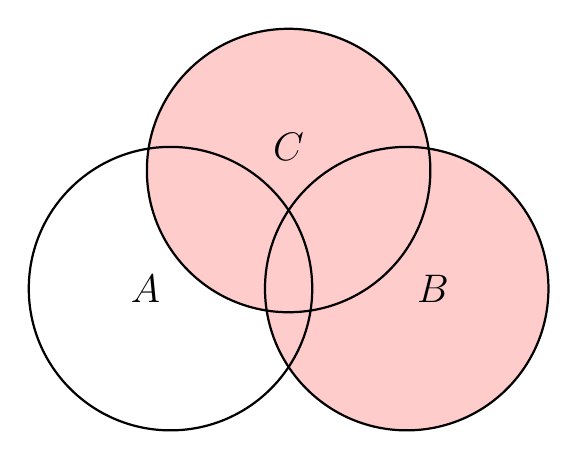
\begin{tikzpicture}
           \fill[red!20] (1.5,0) circle (1.8);  % Set B (shaded)
            \fill[red!20] (0,1.5) circle (1.8);  % Set C (shaded)
            \draw[thick] (-1.5,0) circle (1.8) node[left] {\Large \( A \)};
            \draw[thick] (1.5,0) circle (1.8) node[right] {\Large \( B \)};
            \draw[thick] (0,1.5) circle (1.8) node[above] {\Large \( C \)};
        \end{tikzpicture}
        &
        % Third Venn Diagram
        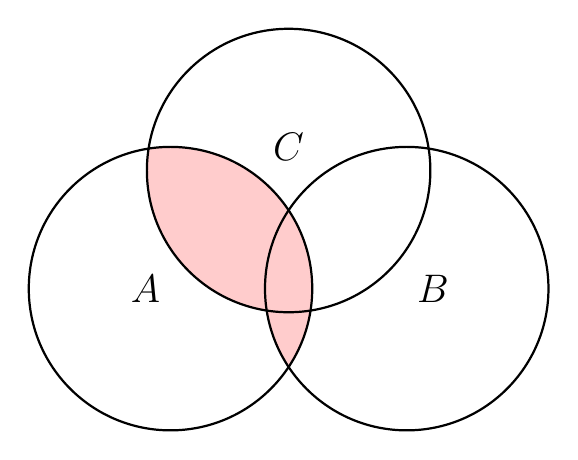
\begin{tikzpicture}
	         % Shade A ∩ (B ∪ C)
	        \begin{scope}
	            \clip (-1.5,0) circle (1.8); % Clip to A
	            \fill[red!20] (1.5,0) circle (1.8); % Fill B
	            \fill[red!20] (0,1.5) circle (1.8); % Fill C
	        \end{scope}
        
            \draw[thick] (-1.5,0) circle (1.8) node[left] {\Large \( A \)};
            \draw[thick] (1.5,0) circle (1.8) node[right] {\Large \( B \)};
            \draw[thick] (0,1.5) circle (1.8) node[above] {\Large \( C \)};
        \end{tikzpicture}
        \\
        & & \\
         \Huge \textbf{$A \cap B$} &         \Huge \textbf{$A \cap C$}  &        \Huge \textbf{$(A \cap B) \cup (A \cap C)$} \\
        % Fourth Venn Diagram
        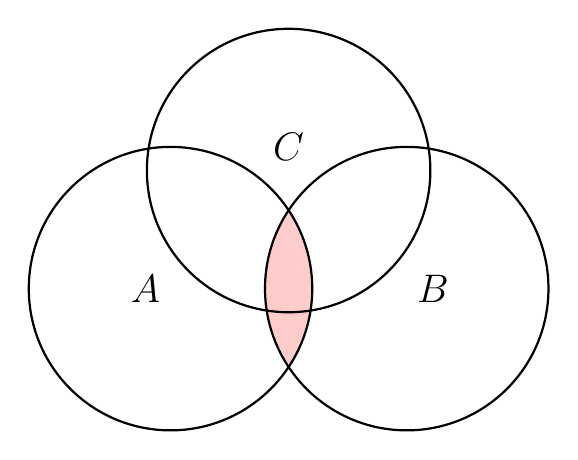
\begin{tikzpicture}
            % Shade A ∩ B
	        \begin{scope}
	            \clip (-1.5,0) circle (1.8); % Clip to A
	            \fill[red!20] (1.5,0) circle (1.8); % Fill B
	        \end{scope}
	        
            \draw[thick] (-1.5,0) circle (1.8) node[left] {\Large \( A \)};
            \draw[thick] (1.5,0) circle (1.8) node[right] {\Large \( B \)};
            \draw[thick] (0,1.5) circle (1.8) node[above] {\Large \( C \)};
        \end{tikzpicture}
        &
        % Fifth Venn Diagram
        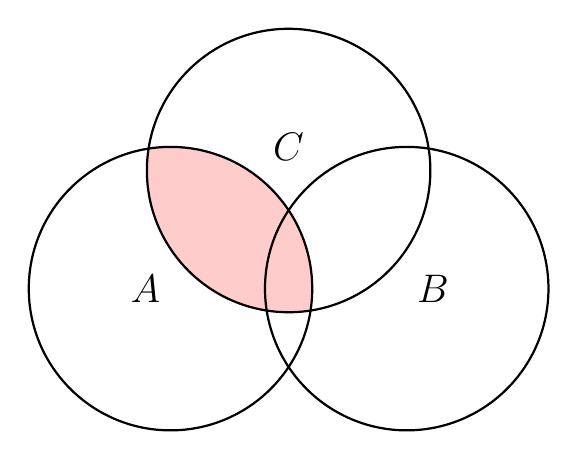
\begin{tikzpicture}
             % Shade A ∩ C
	        \begin{scope}
	            \clip (-1.5,0) circle (1.8); % Clip to A
	            \fill[red!20] (0,1.5) circle (1.8); % Fill C
	        \end{scope}
	        
            \draw[thick] (-1.5,0) circle (1.8) node[left] {\Large \( A \)};
            \draw[thick] (1.5,0) circle (1.8) node[right] {\Large \( B \)};
            \draw[thick] (0,1.5) circle (1.8) node[above] {\Large \( C \)};
        \end{tikzpicture}
        &
        % Sixth Venn Diagram
        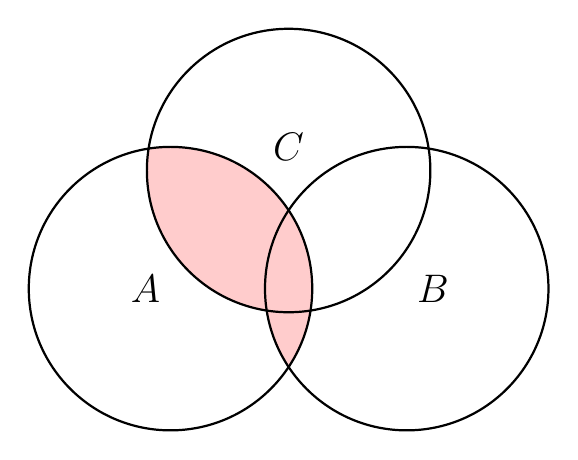
\begin{tikzpicture}
	        \begin{scope}
	            \clip (-1.5,0) circle (1.8); % Clip to A
	            \fill[red!20] (1.5,0) circle (1.8); % Fill B
	            \fill[red!20] (0,1.5) circle (1.8); % Fill C
	        \end{scope}
        
            \draw[thick] (-1.5,0) circle (1.8) node[left] {\Large \( A \)};
            \draw[thick] (1.5,0) circle (1.8) node[right] {\Large \( B \)};
            \draw[thick] (0,1.5) circle (1.8) node[above] {\Large \( C \)};
        \end{tikzpicture}
    \end{tabular}
    }
\end{frame}


\begin{frame}{Solution to Group Exercise \#3 }
\footnotesize 
\colorbox{red!30}{\textbf{Problem.}}  The distributive properties for sets are 
    \[ A \cup (B \cap C) = (A \cup B) \cap (A \cup C), \qquad \text{and} \qquad  A \cap (B \cup C) = (A \cap B) \cup (A \cap C). \]
Prove that the second identity above holds.  Hint: You may want to refer back to Theorem 7.2.	

 \onslide<2->{\colorbox{green!30}{\textbf{Solution.}} }

\begin{align*}
 \onslide<2->{A \cap (B \cup C) &= \set{x: x \in A \text{ and } x \in B \cup C} && \scripttext{(by def. intersection $\cap$)}} \\
 \onslide<3->{&= \set{x: x \in A \text{ and } (x \in B \text{ or }  x \in C) } && \scripttext{(by def. union $\cup$)}} \\
 \onslide<4->{&= \set{x: (x \in A \text{ and } x \in B) \text{ or }  (x \in A \text{ and } x \in C) } && \scripttext{(by distributive prop.; Thm 7.2)}} \\
 \onslide<5->{&= \set{x: (x \in A \cap B) \text{ or }  (x \in A \cap C)} && \scripttext{(by def. intersection $\cap$)}} \\
 \onslide<6->{&= (A \cap B) \cup (A \cap C) && \scripttext{(by def. union $\cup$)}}
\end{align*}

 \onslide<7->{\colorbox{blue!30}{\textbf{Remark.}} We used the distributive property for \textit{Boolean Algebra} (from Theorem 7.2) to prove the distributive property for \textit{sets}.}
\end{frame}



\begin{frame}{Solution to Group Exercise \#4 }
\small 

\colorbox{red!30}{\textbf{Problem.}}  How many integers in the range 1 to 1000 (inclusive) are divisible by 2 or by 5?  Justify your answer.

\vfill 

\colorbox{green!30}{\textbf{Sketch of Solution.}} 
Let
%
\begin{align*}
A &\defeq \set{x \in \mathbb{Z} : 2|x} \\
B &\defeq \set{x \in \mathbb{Z} : 5|x} 
\end{align*}
%
We want $|A \cup B|$.  That's hard to calculate. \\

However, we have
\begin{align*}
|A| &= 500 && \scripttext{(by skip counting)} \\
|B| &= 200 && \scripttext{(by skip counting)} \\
|A \cap B| &= \bigg| \set{x \in \mathbb{Z} : 10|x} \bigg| = 100 && \scripttext{(by skip counting)} 
\end{align*}

Now we apply the identity to find
\begin{align*}
|A \cup B|  &= |A| + |B| - |A \cap B| \\
			&= 500 + 200 - 100 = 600.
\end{align*}


\end{frame}


\end{document}
